% Recommended preamble:
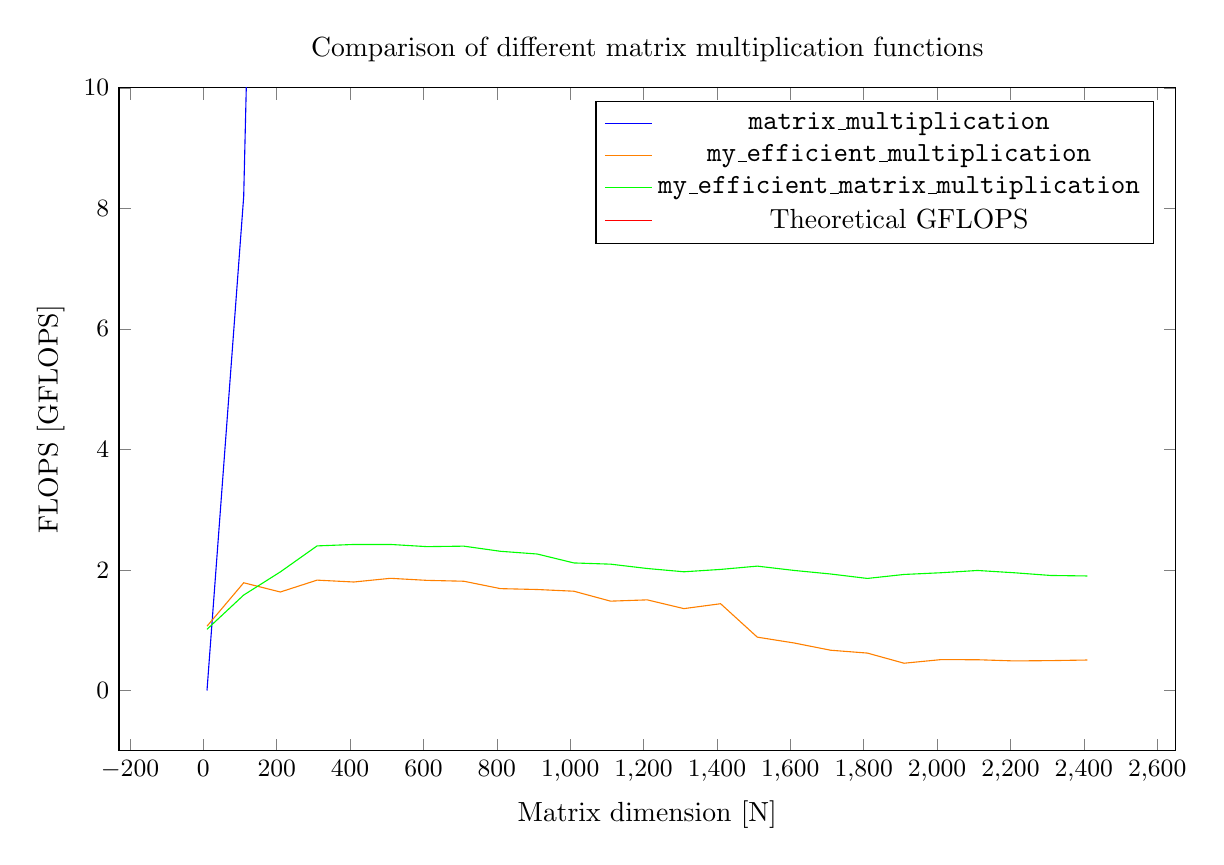
\begin{tikzpicture}
\begin{axis}[width={15cm}, height={10cm}, xlabel={Matrix dimension [N]}, ylabel={FLOPS [GFLOPS]}, title={Comparison of different matrix multiplication functions}, legend={north east}, ymax={10},    scaled ticks=false,   % Prevents scientific notation or compression in the ticks
    xticklabel style={/pgf/number format/fixed},  % Ensures tick labels are printed in a fixed format without rounding
    xticklabel style={/pgf/number format/precision=0},  % Rounds the numbers to integers to avoid crowding
    ticklabel style = {font=\small},  % Reduces the size of the tick labels to prevent overlap
    ]
    \addplot[no marks, blue]
        table[row sep={\\}]
        {
            \\
            10.0  0.0023079523961738765  \\
            110.0  8.194097294901313  \\
            210.0  33.72498893859692  \\
            310.0  63.67891003491642  \\
            410.0  83.20933205921395  \\
            510.0  121.0965154318156  \\
            610.0  114.15410635879024  \\
            710.0  148.78480554332117  \\
            810.0  128.77979771936313  \\
            910.0  46.69649114974178  \\
            1010.0  149.39668260804913  \\
            1110.0  185.67318648613312  \\
            1210.0  139.70476585037548  \\
            1310.0  140.825722756572  \\
            1410.0  157.08443564188434  \\
            1510.0  189.98083748640684  \\
            1610.0  201.73749401185015  \\
            1710.0  238.16347699049706  \\
            1810.0  184.7190920582196  \\
            1910.0  236.60746961674465  \\
            2010.0  189.07665556113673  \\
            2110.0  208.35783211953395  \\
            2210.0  211.28693733594844  \\
            2310.0  220.6979894130633  \\
            2410.0  185.3414228183199  \\
        }
        ;
    \addplot[no marks, orange]
        table[row sep={\\}]
        {
            \\
            10.0  1.0689470871191875  \\
            110.0  1.7891119566042895  \\
            210.0  1.6363952973381144  \\
            310.0  1.833138380472606  \\
            410.0  1.8019750452823982  \\
            510.0  1.8633233611285047  \\
            610.0  1.829149502012656  \\
            710.0  1.814902720882529  \\
            810.0  1.691969911709576  \\
            910.0  1.67758644720142  \\
            1010.0  1.649210445467428  \\
            1110.0  1.4844659134712057  \\
            1210.0  1.50570400213252  \\
            1310.0  1.36048195288819  \\
            1410.0  1.441815509625949  \\
            1510.0  0.8870844660154257  \\
            1610.0  0.7907230876381947  \\
            1710.0  0.6699917469778933  \\
            1810.0  0.622945715952708  \\
            1910.0  0.4545396698327844  \\
            2010.0  0.5141040422999137  \\
            2110.0  0.5125469619014145  \\
            2210.0  0.49265788054693666  \\
            2310.0  0.497771062036038  \\
            2410.0  0.5078183160369875  \\
        }
        ;
    \addplot[no marks, green]
        table[row sep={\\}]
        {
            \\
            10.0  1.017293997965412  \\
            110.0  1.5855298659744814  \\
            210.0  1.9699571431686191  \\
            310.0  2.4009089137903974  \\
            410.0  2.424738077028364  \\
            510.0  2.4250974800940805  \\
            610.0  2.3888349809526823  \\
            710.0  2.3969416901613645  \\
            810.0  2.3114564185518116  \\
            910.0  2.2665805230657363  \\
            1010.0  2.1183366990174863  \\
            1110.0  2.098103432813833  \\
            1210.0  2.02596145383276  \\
            1310.0  1.9715949457443354  \\
            1410.0  2.010909758662662  \\
            1510.0  2.065411932336678  \\
            1610.0  1.9941957000538721  \\
            1710.0  1.9348035190308683  \\
            1810.0  1.86114085663287  \\
            1910.0  1.9272390772083445  \\
            2010.0  1.9553976471457613  \\
            2110.0  1.993427896663581  \\
            2210.0  1.9556294361633033  \\
            2310.0  1.9104629902084065  \\
            2410.0  1.9020792743764794  \\
        }
        ;
    \addplot[no marks, red]
        table[row sep={\\}]
        {
            \\
            10.0  288.0  \\
            110.0  288.0  \\
            210.0  288.0  \\
            310.0  288.0  \\
            410.0  288.0  \\
            510.0  288.0  \\
            610.0  288.0  \\
            710.0  288.0  \\
            810.0  288.0  \\
            910.0  288.0  \\
            1010.0  288.0  \\
            1110.0  288.0  \\
            1210.0  288.0  \\
            1310.0  288.0  \\
            1410.0  288.0  \\
            1510.0  288.0  \\
            1610.0  288.0  \\
            1710.0  288.0  \\
            1810.0  288.0  \\
            1910.0  288.0  \\
            2010.0  288.0  \\
            2110.0  288.0  \\
            2210.0  288.0  \\
            2310.0  288.0  \\
            2410.0  288.0  \\
        }
        ;
        \addlegendentry {\texttt{matrix\_multiplication}}
        \addlegendentry {\texttt{my\_efficient\_multiplication}}
        \addlegendentry {\texttt{my\_efficient\_matrix\_multiplication}}
        \addlegendentry {Theoretical GFLOPS}        
\end{axis}
\end{tikzpicture}
